\chapter{二类疾病标记物定位的实验评估}\label{sec:experiments}
在第\ref{sec:method}章中,本文详细介绍了本文提出的模型、训练策略、损失函数等内容。本章将使用本文提出的模型处理二类疾病标记物定位问题。本文首先在\ref{sec:exper_ds_intro}小节中介绍二类糖尿病性视网膜病变数据集和二类模拟皮肤病病变数据集。在\ref{sec:exper_evaluation_metrics}小节中,本文将说明本章实验所选择的评价标准及其原因。\ref{sec:exper_setting}小节将会介绍本章的实验设置。在\ref{sec:bin_dr_ds_experiment}小节和\ref{sec:bin_simulated_ds_experiment}小节中,本章将分别在以上两个数据集上对比本文提出的方法、CAM以和Grad-CAM的疾病标记物定位性能。在\ref{sec:g_c_g_d_g_d_c_comparsion}小节中,本章通过分别去掉本文提出的模型中的CNN分类器和判别器的方式设计消融实验来探究本文提出的模型中的两个子模块所扮演的角色。在\ref{sec:indirect_quantitative_evaluation}小节中,本章通过对比二类糖尿病性视网膜病变数据集和经过编码器-解码器的二类糖尿病性视网膜病变数据集的分类情况来间接定量评估本文提出的方法的性能。在\ref{sec:dis_arch}小节中,本章将探究不同的判别器网络结构下,本文提出的模型的性能,以期读者能对判别器的模型结构有更为深刻的认识。\ref{sec:hyper_paras}小节将设置不同的超参数$\lambda_{1}$和$\lambda_{2}$组合,来探究本文提出的模型的鲁棒性。
\section{数据集介绍}\label{sec:exper_ds_intro}
在本章中,本文将详细介绍本文提出的模型在处理二类疾病标记物定位问题时的性能表现。在\ref{sec:usually_ds_intro}小节中,本文介绍了包括眼底病变数据集和黑色素瘤皮肤病病变数据集在内的多个可用于疾病标记物定位任务的常见数据集。黑色素瘤皮肤病病变图像中的疾病标记物分布较为集中,都聚集于某一区域,异常区域所占比例通常在1/3以上,疾病标记物尺寸也都偏大,还没有专门的正常图像。考虑到本文的研究内容是在疾病标记物分布比较分散、疾病标记物尺寸大小不一的情况下精确定位疾病标记物,本文将在疾病标记物具有以上特点的二类糖尿病性视网膜病变数据集和二类模拟皮肤病病变数据集上评估本文提出的方法定位疾病标记物的表现。
\subsection{二类糖尿病性视网膜病变数据集}\label{subsec:bin_dr_ds}
本文二类糖尿病性视网膜病变数据集是来自Kaggle糖尿病性视网膜病变数据集(相关描述请参见\ref{subsec:original_dr_dataset_intro}小节),该数据集由从原始Kaggle糖尿病性视网膜病变数据集中随机选择出来的2,101张异常图像和2,101张正常图像组成,图像尺寸大小为128$\times$128。由于原始Kaggle眼底图像中均存在没有信息的四个黑角,为了去除这些冗余信息,我们充分利用了眼底图像中视网膜边界十分接近圆形这一特点,我们先提取了视网膜边界再取其最大内接矩形,最后将图像尺寸大小重新调整到128$\times$128。

该数据集中的部分图像示例如图\ref{subfig:bin_dr_ds_example}所示。可以发现,图像中明显比周围要亮的圆形区域为视盘,为眼底图像公有结构,有些图像中视盘在左边,有些视盘在右边,这是因为有些图像是左眼眼底图像,而有些是右眼眼底图像。眼底图像还含有丰富的血管,呈现一种随机走向。图像之间的背景亮度有较大差别,比如,图中第一行、第三列图像背景较亮,而第二列、第一行图像背景较暗。就疾病标记物本身来说,也呈现一种分散、大小不一、极少数难以被察觉的特点,而且疾病标记物本身的颜色与背景颜色比较相近,比如图中的第二列、第三行和第一列、第三行图像,导致这些疾病标记物很容易与背景相混淆,这些特点都表明在该数据集上完成疾病标记物定位任务极具挑战性。由于在该数据集上进行像素级标注代价高昂,我们选择随机选出40张眼底图像并邀请两位眼科医生对其进行像素级标注,用于后续章节中对实验的定量分析。

\begin{figure}[h!]
	\centering
	\begin{subfigure}{0.48\textwidth}
		\centering
		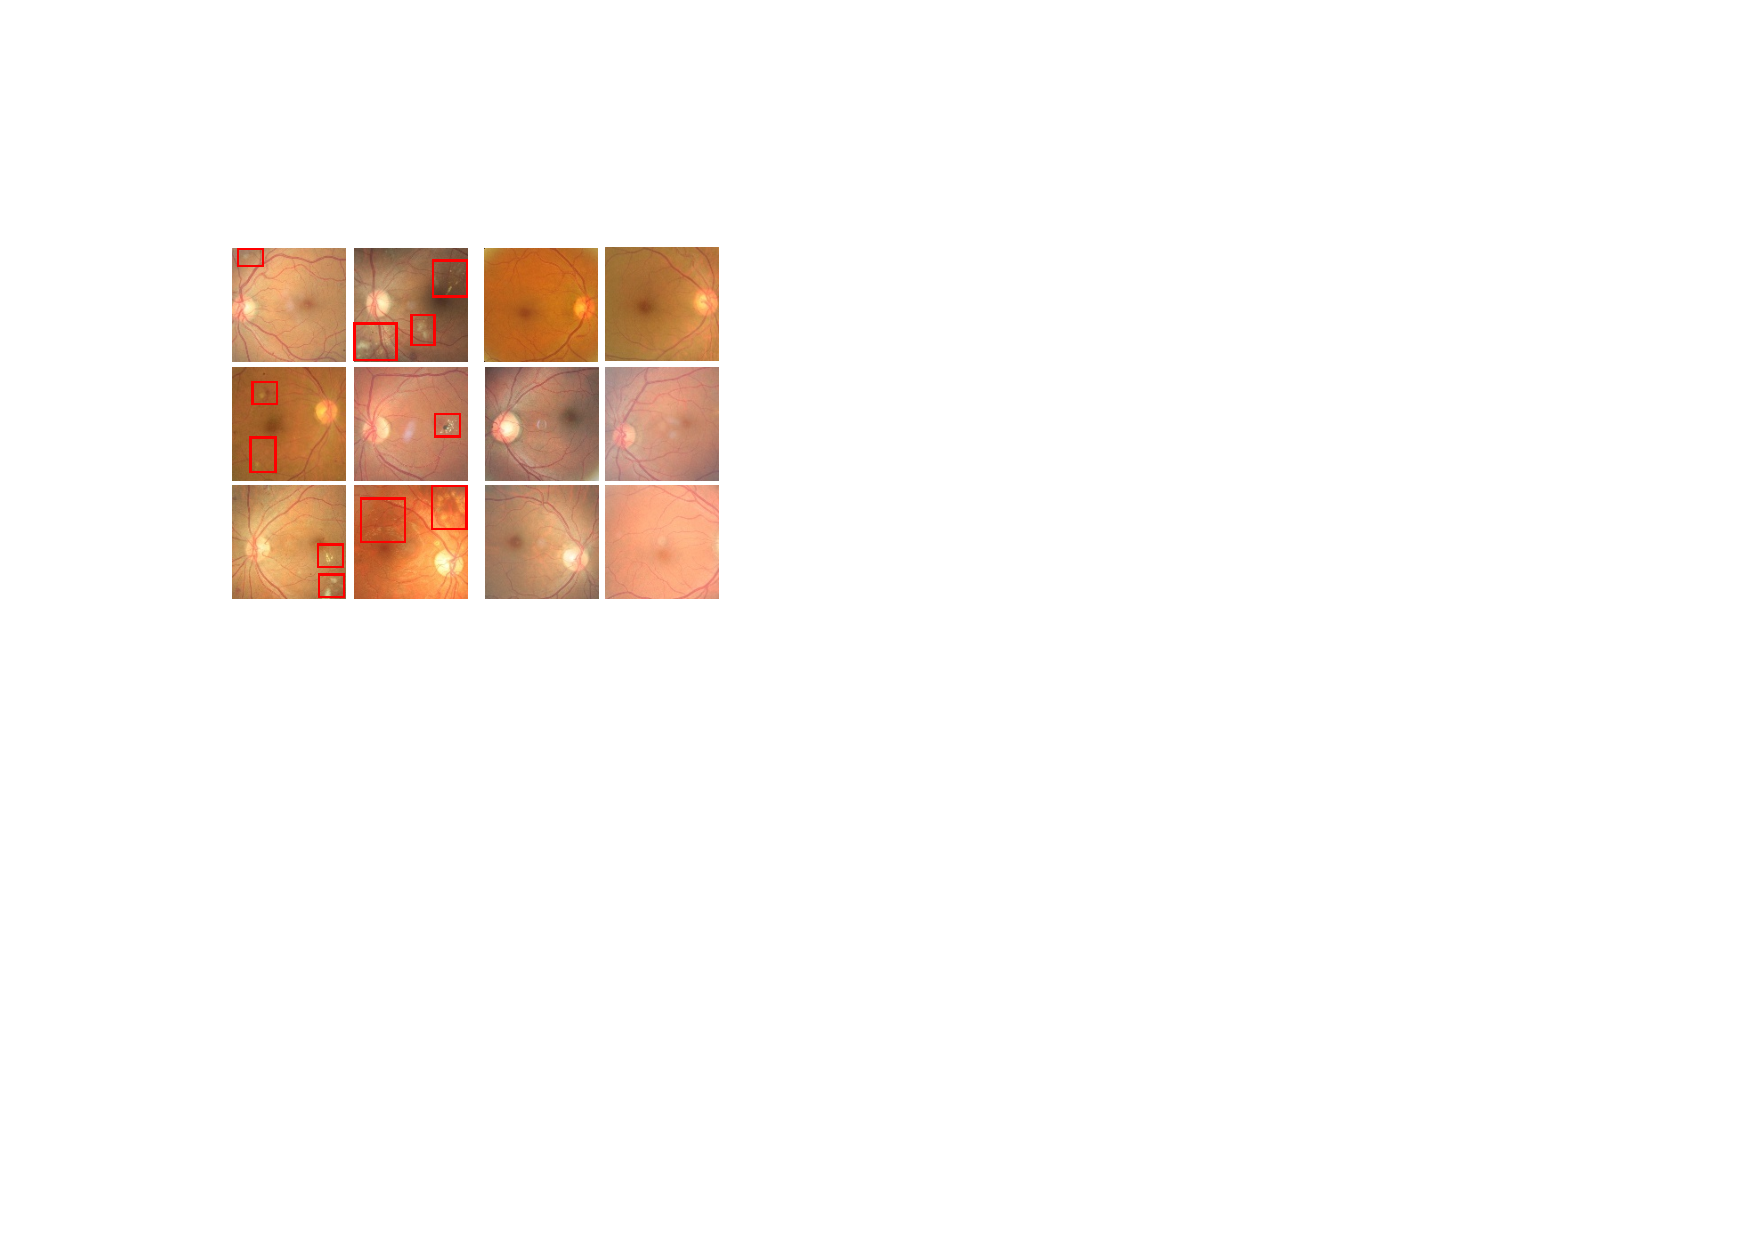
\includegraphics[width=1\textwidth]{figure/bin_dr_ds_example}
		\caption{二类糖尿病性视网膜病变数据集部分图像示例(第1列和第2列是异常图像,第3列和第4列是正常图像)。}
		\label{subfig:bin_dr_ds_example}
	\end{subfigure}
	\quad
	\begin{subfigure}{0.48\textwidth}
		\centering
		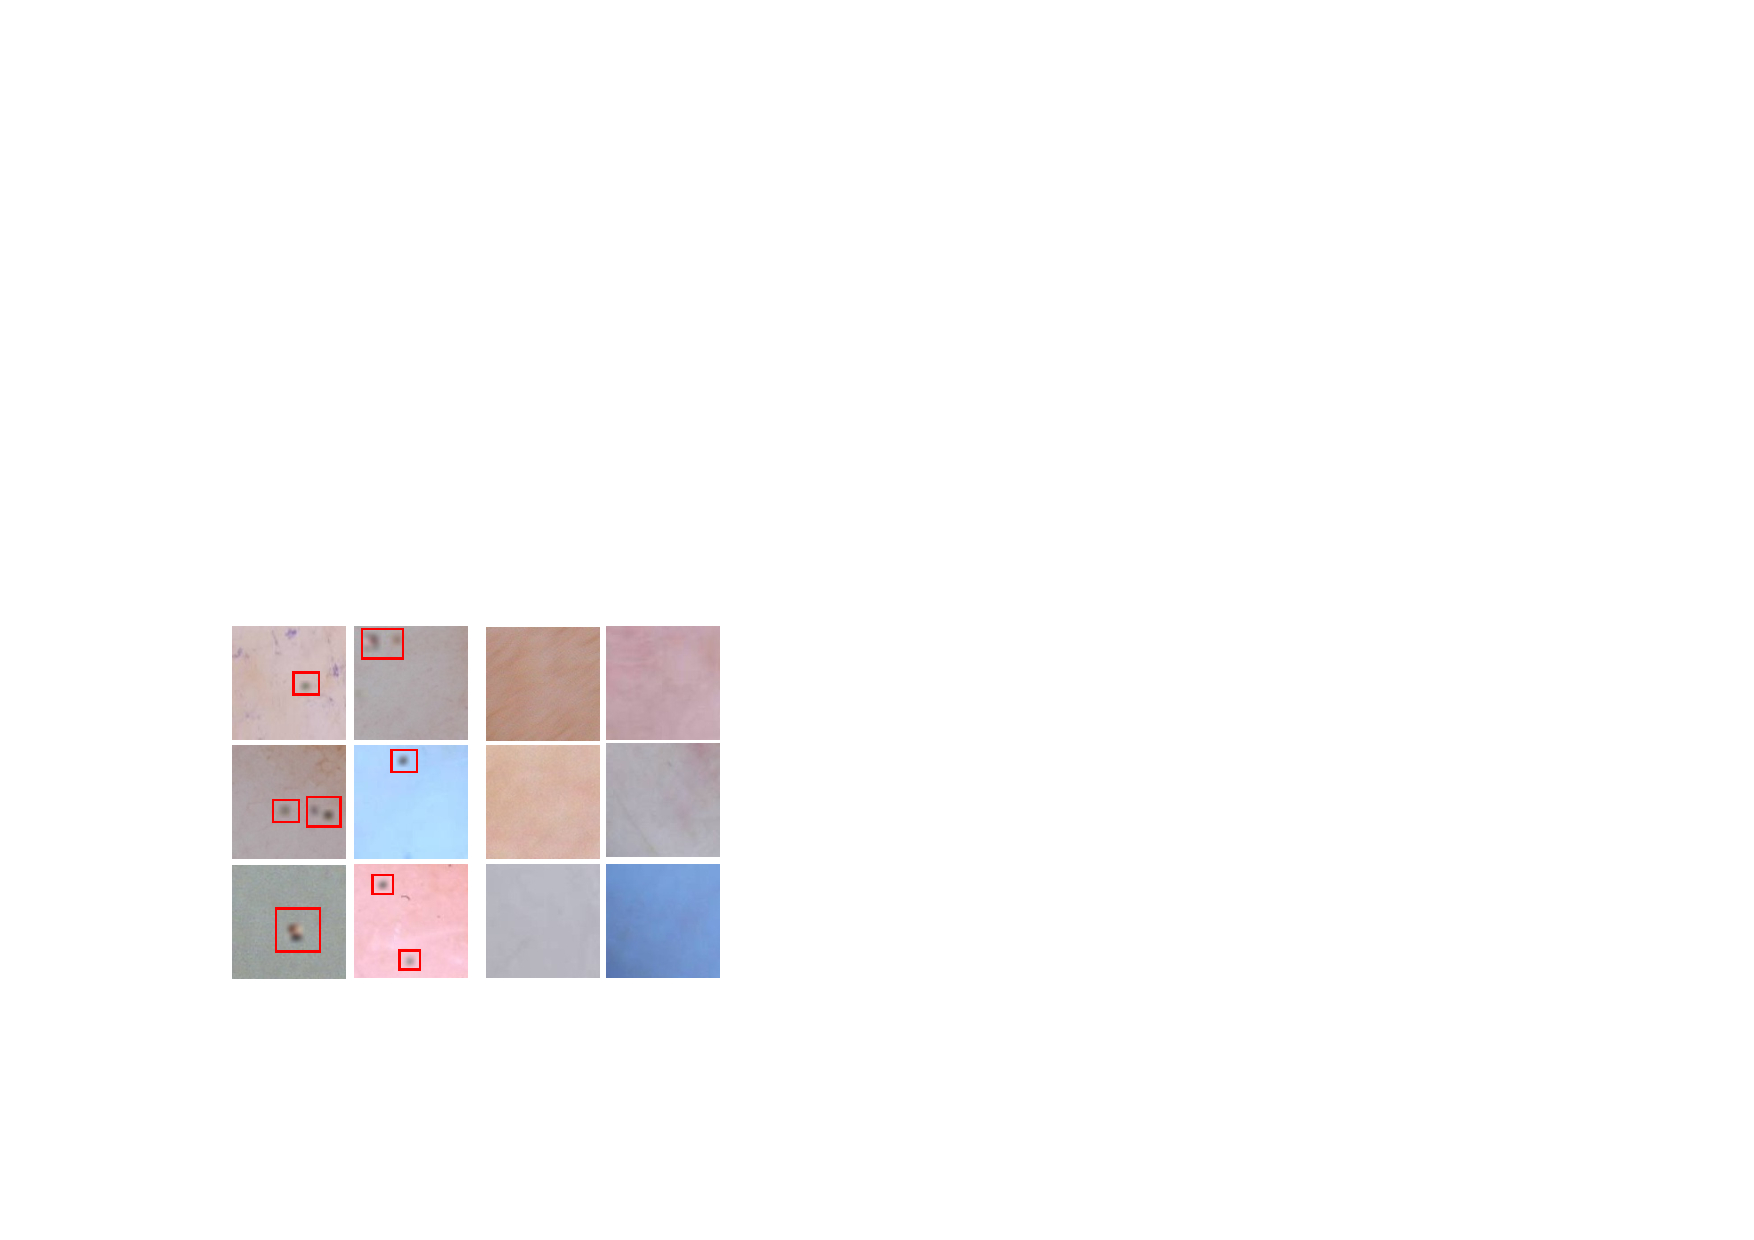
\includegraphics[width=1\textwidth]{figure/bin_simulate_skin_example}
		\caption{二类模拟皮肤病病变数据集部分图像示例(第1列和第2列是异常图像,第3列和第4列是正常图像)。}
		\label{subfig:bin_simulate_skin_example}
	\end{subfigure}
	\caption[本章实验数据集部分示例图像]{二类糖尿病性视网膜病变数据集和二类模拟皮肤病病变数据集中的部分示例图像(红色矩形框表示疾病标记物)。}
	\label{mul_fig:bin_ds_example}
\end{figure}
\subsection{二类模拟皮肤病病变数据集}\label{subsec:bin_simulated_skin_ds}
二类模拟皮肤病病变数据集包含带有模拟疾病标记物的皮肤图像。为了生成这个数据集,我们首先从一个皮肤镜图像数据集~\cite{codella2018skin}(原始数据集相关内容介绍可参见\ref{subsec:original_dermatoscope_ds_intro}小节)中提取了2,920张图像尺寸大小为128$\times$128的正常图像(实际上是通过滑动窗口方式得到的图像区域块)。为了模拟真实皮肤图像中疾病标记物的数量、大小和所在位置的随机变化,我们通过随机参数控制,在每个模拟皮肤图像的一定范围内随机生成这些参数的值。更具体地说,对于每张异常图像,从Image-Net数据集~\cite{deng2009imagenet}中随机选择一到三张图像,并将其调整为尺寸大小为4$\times$4、8$\times$8或16$\times$16的缩略图。再将缩略图嵌入到皮肤图像中,最后将其局部平滑作为模拟疾病标记物。最终,二类模拟皮肤病病变数据集中共有异常图像1,310张,正常图像1,460张。注意,此数据集中的所有异常图像的模拟疾病标记物都有像素级的标注。该数据集中的部分图像示例如图\ref{subfig:bin_simulate_skin_example}所示。

从图\ref{subfig:bin_simulate_skin_example}中可以看出,二类模拟皮肤病病变数据集中背景差异比较大,主要表现在颜色和亮度,比如图中第二行、第三列图像背景为红色,较亮,而第一行、第二列图像背景较暗。注意,由于本文对于所有异常图像中的疾病标记物都做了局部平滑处理,最为明显的特点是其边界比较模糊。再加上引入了疾病标记物大小、数量和位置这三个随机变化量,这大大增加了模拟疾病标记物的真实性。与二类糖尿病性视网膜病变数据集相比,二类模拟皮肤病病变数据集的最大优势在于拥有所有疾病标记物的像素级标注,可以全面评估不同方法定位疾病标记物的性能,这也是设置该数据集的意义所在。
\section{评价标准}\label{sec:exper_evaluation_metrics}
在\ref{sec:evaluation_metrics}小节中,本文分别介绍了ROC曲线和P-R曲线及其各自AUC,并说明了在正负样本比例悬殊较大情况下,P-R曲线更能反映出系统的真实分类性能。从表\ref{tab:bin_ds_pixel_freqs}可以看出,无论是二类糖尿病性视网膜病变数据集还是二类模拟皮肤病病变数据集,异常像素和正常像素数量之间的比例存在巨大悬殊最高达到88:1(二类糖尿病性视网膜病变数据集),故接下来的实验均采用P-R曲线及其AUC作为主要评价标准,ROC曲线也会在本文附录\ref{chapter:append1}中进行展示,以更为全面地评估实验。本章还引入特异性(Specificity)和召回率(Recall)分别衡量编码器-解码器对正常图像输入的保持能力和对异常图像输入的转化能力,以间接评估本文提出的方法定位疾病标记物的性能。
\begin{table}[h]
	\centering
	\caption[本章实验数据集正负像素数量统计表]{二类糖尿病性视网膜病变数据集和二类模拟皮肤病病变数据集正负像素数量统计表。}
	\label{tab:bin_ds_pixel_freqs}
	\begin{tabular}{c|c|c|c}
		\toprule[2pt]
		数据集名称 & 正常像素数量 & 异常像素数量 & 比例 \\
		\midrule[2pt]
		二类糖尿病性视网膜病变数据集&  643,837 & 11,523 & $\simeq$ 56:1 \\ \hline
		二类模拟皮肤病病变数据集 & 21,222,487 & 240,553 & $\simeq$ 88:1 \\
		\bottomrule[2pt]
	\end{tabular}
\end{table}
\section{实验设置}\label{sec:exper_setting}
本文所有实验相关代码实现均采用当前流行的深度学习框架PyTorch\footnote{https://pytorch.org/}。编码器-解码器选择一个经过修改的U-Net~\cite{iglovikov2018ternausnet}(网络结构见图\ref{fig:auto_encoder_architecture})。CNN分类器采用Resnet-18(模型结构见图\ref{subfig:classifier_architecture}),判别器使用一个7层卷积神经网络(模型结构见图\ref{subfig:discrimintor_architecture}),其中前4层是下采样卷积层。GAN采用WGAN-GP。为了让U-Net更好地重构输入图像,本文先将编码器-解码器在两个数据集上进行预训练。

在预处理阶段,在图像数据送入模型训练之前,我们将输入减去0.5随后除以0.5,将输入变换到[-1,1]。在实验超参数设定方面,WGAN-GP中的梯度惩罚系数$\lambda$被设置为10(与WGAN-GP原文中一致)。本文使用Adam优化器更新网络参数,其中,对于CNN分类器,$\beta1$和$\beta2$分别设为0.9和0.999,对于生成器和判别器,$\beta1$和$\beta_2$分别设为0.3和0.9,默认学习率取0.0002,训练每次迭代取32张图像。对于所有的测试,$\lambda_1$ = 0.4和$\lambda_{2}$ = 10.0,本文提出的模型默认在数据集上训练500轮。

请注意,我们的目标是通过图像级标签从已有图像中搜索和定位疾病标记物,而不是训练模型从新图像中寻找疾病标记物。因此,对于每个数据集,所有的图像都被用来训练我们的模型,然后对模型进行定性和定量的评估。因此,我们没有设置额外的验证集,将在相同的数据集上训练和评估我们的模型。基于同样的原因,在训练阶段,我们也没有采用随机翻转、随机裁剪、随机加入噪音等数据增广手段。在生成P-R曲线之前,定位结果的热图被归一化为[0,1]。

\section{在二类糖尿病性视网膜病变数据集上的疾病标记物定位}\label{sec:bin_dr_ds_experiment}
本节将展示本文提出的模型在二类糖尿病性视网膜病变数据集上的实验结果,本文提出的模型将与两种CNN可视化方法(CAM和Grad-CAM)作比较。

如果使用CAM或者Grad-CAM来定位异常图像中的疾病标记物,本身均需要分两步完成。首先需要训练一个分类器,再通过找到异常图像中的判别性区域来间接定位疾病标记物。本文将ResNet-18作为CAM和Grad-CAM可视化的目标CNN分类器。为了保持实验设置的一致性,本文同样使用数据集中的所有图像来训练ResNet-18分类器,除非单独说明,本文后续所有关于CAM和Grad-CAM的相关实验结果均在此设置下完成。在二类糖尿病性视网膜病变数据集上训练ResNet-18后,分类器最终的分类准确率达到了100$\%$,说明分类器已经能够很好地学到了疾病标记物的特征,也排除了ResNet-18较差的分类性能导致较差的定位结果这一可能。由于Grad-CAM可可视化任意层输出的特征图,如图\ref{fig:retinal_image_res}所示,本文展示出了使用Grad-CAM可视化中间卷积层输出特征(第4列)和最后一层卷积层输出特征(第5列)得到的疾病标记物定位热图。
\begin{figure}[h]
	\centering
	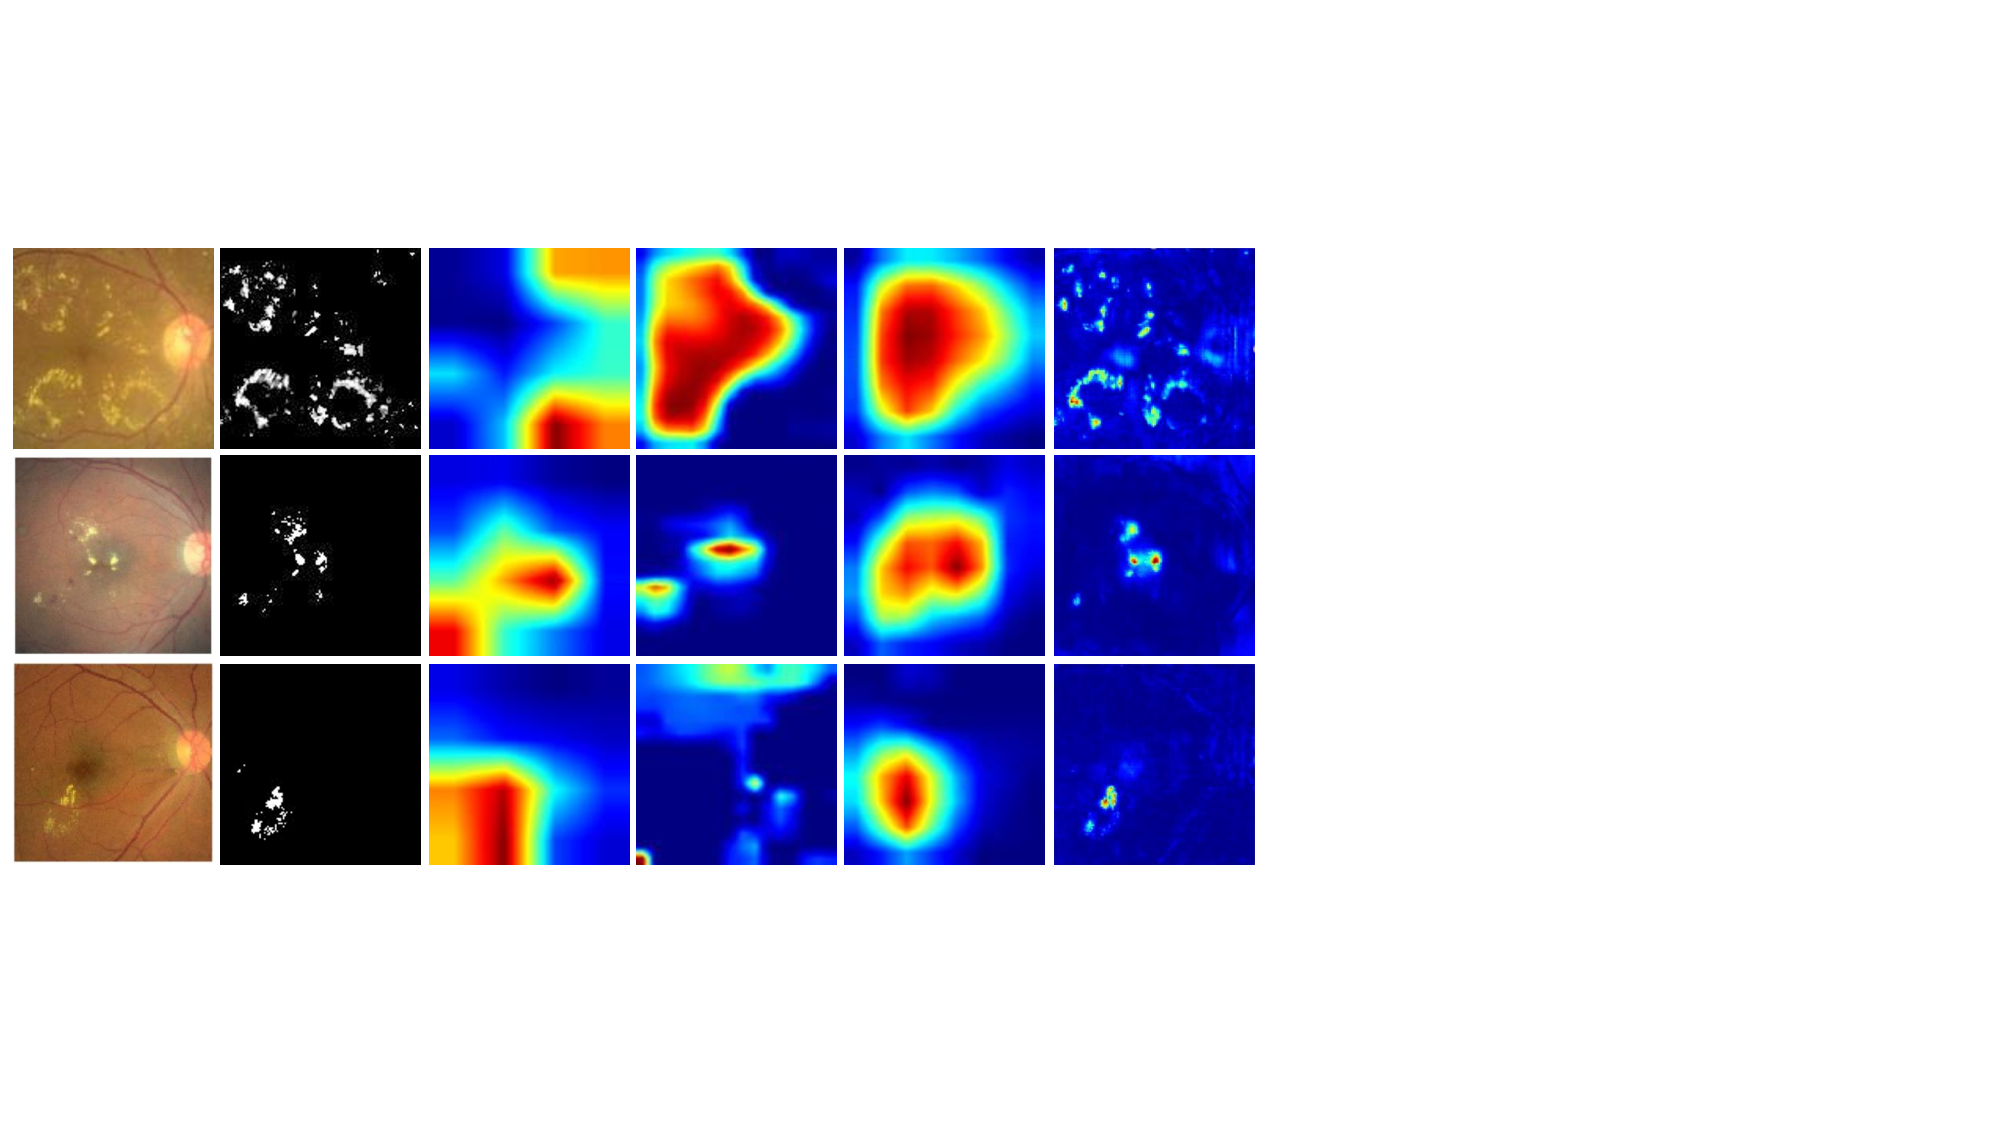
\includegraphics[width=1.0\textwidth]{figure/retinal_image_res.pdf}
	\caption[在二类糖尿病性视网膜病变数据集上疾病标记物定位热图对比]{在二类糖尿病性视网膜病变数据集上疾病标记物定位热图对比。}
	\label{fig:retinal_image_res}
\end{figure}

如图\ref{fig:retinal_image_res}所示,图中第1列表示原始异常图像,第2列表示其像素级标注,第3列表示CAM可视化得到的定位热图,第4列表示使用Grad-CAM可视化分类器中间卷积层输出特征得到的定位热图(Grad-CAM-1),第5列表示使用Grad-CAM可视化分类器最后一层卷积层输出特征得到的定位热图(Grad-CAM-2),第6列是本文提出的模型得到的定位热图。对于第3-6列的热图,图中某一区域颜色越红,表示该区域为疾病标记物的可能性越高。蓝色表示的意义与红色相反,表示其所在区域是疾病标记物的可能性越低。以上颜色代表的意义同样适用于下文所有热图。

从图中第3列定位结果可以看出,虽然CAM发现的疾病标记物或者说异常区域最多,但是CAM也将周边正常区域作为疾病标记物的一部分,也就是说,CAM只能定位到部分疾病标记物。这是因为CAM在可视化过程中需要将最后一个卷积层的输出(4$\times$4)上采样到原图像大小(128$\times$128)。Grad-CAM作为CAM的扩展,它允许我们从多个层生成可视化热图,例如,中间卷积层(第4列,Grad-CAM-1)和最后一层卷积层(第5列,Grad-CAM-2)。虽然Grad-CAM-1在第2行图像中获得了相对准确的疾病标记物定位结果,但同时也将正常区域误认作包含疾病标记物的异常区域,更多的是其结果要么不够精确(第1行),要么不够准确(第2行和第3行)。注意到在第3行中,Grad-CAM-1几乎没有定位到疾病标记物,这很可能是中间卷积层输出特征图的语义性不够高,中间卷积层输出特征图中只有极少数包含与疾病标记物相关的判别性特征。但与CAM相比,Grad-CAM-1还是实现了更为精确的定位结果,证明了其优于CAM的性能。Grad-CAM-2(第5列)标记的区域和CAM(第3列)没有太大区别。相比之下,本文提出的方法对形状不规则、分布分散的疾病标记物进行了更精确地定位(第6列),从定性分析角度证明了其优于CAM和Grad-CAM的性能。
\begin{figure}[h!]
	\centering
	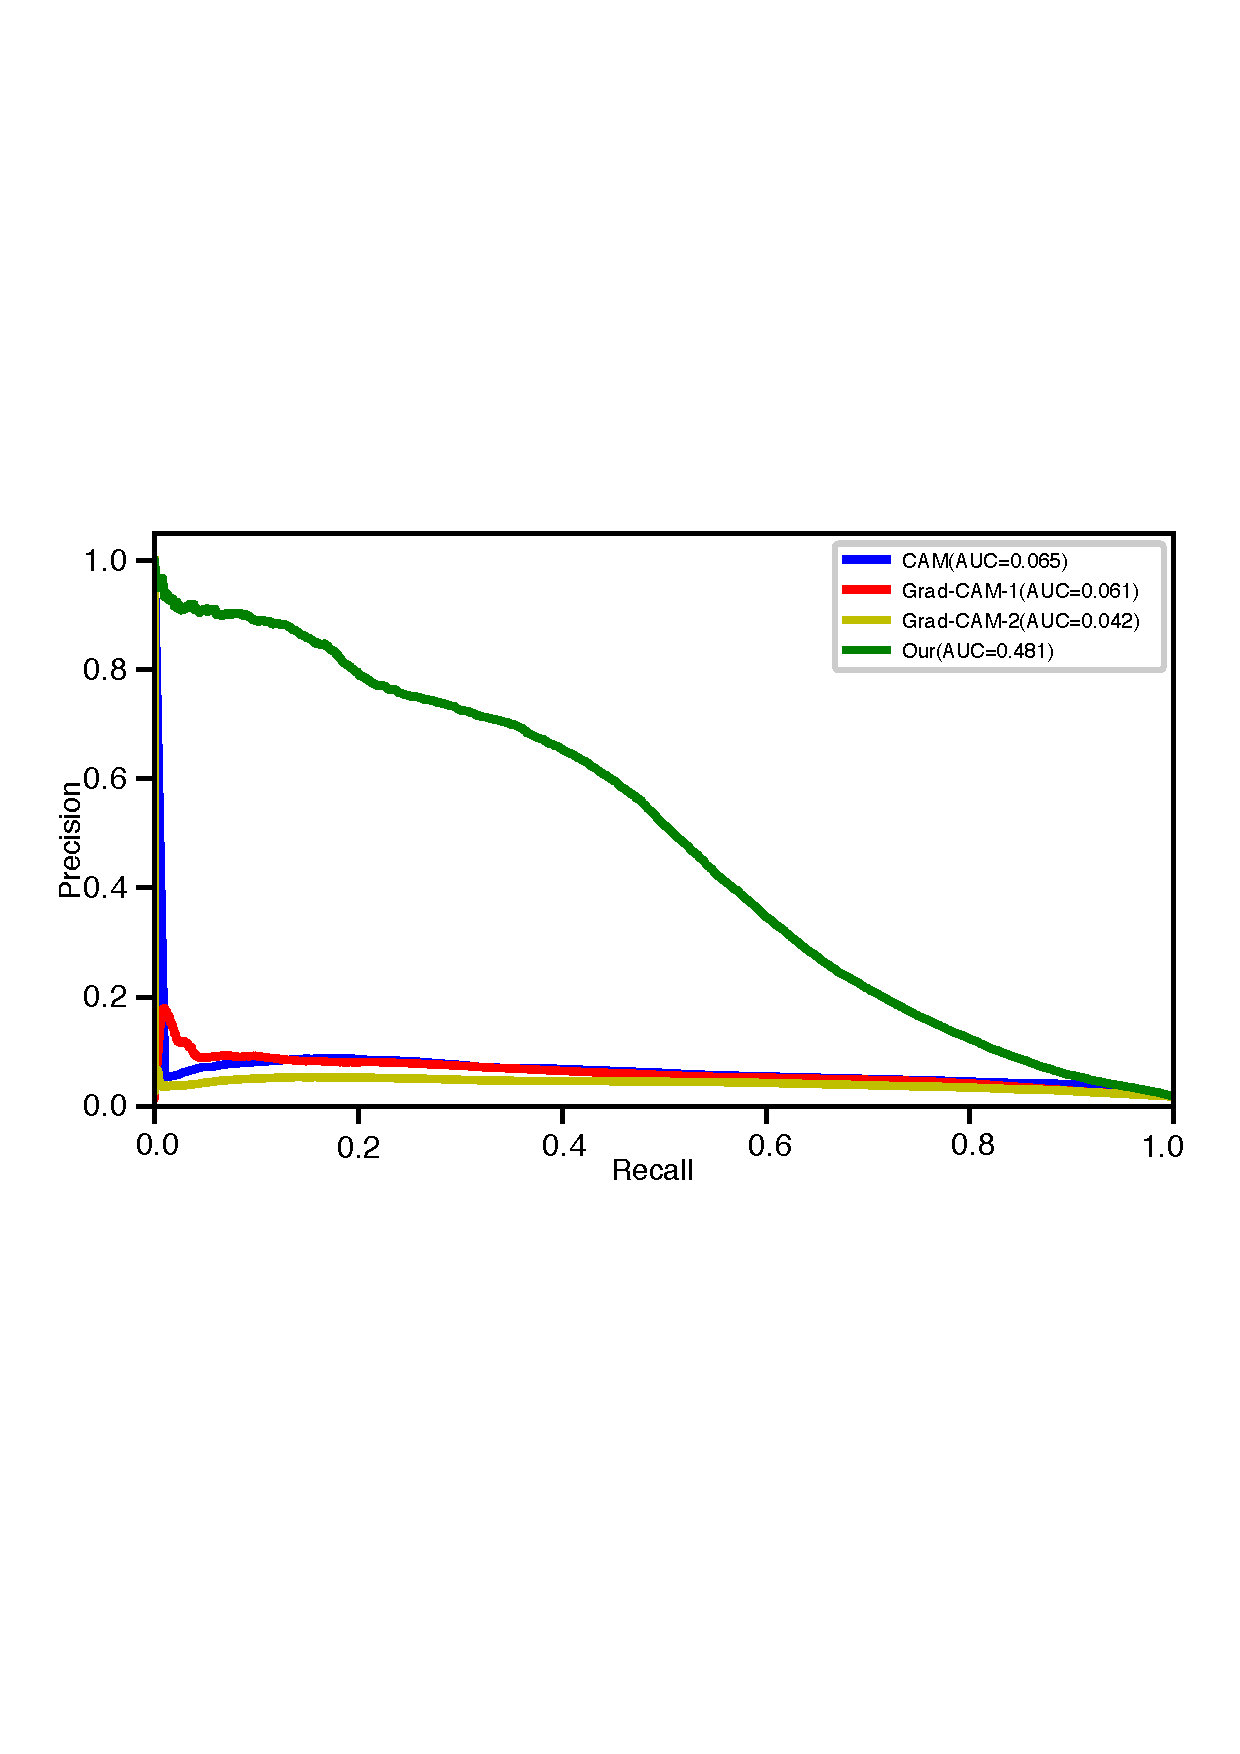
\includegraphics[width=0.7\textwidth]{figure/pr_curve_retinal_image/pr_curve}
	\caption[在40张糖尿病性视网膜病变图像上P-R曲线对比]{在40张糖尿病性视网膜病变图像上P-R曲线对比。}
	\label{fig:retinal_image_pr_curve}
\end{figure}

除了上述定性分析角度外,本文还充分利用二类糖尿病性视网膜病变数据集中的40张像素级标注图像,完成了对每种方法的定量分析,本文提出的模型、CAM、Grad-CAM-1和Grad-CAM-2的P-R曲线如图\ref{fig:retinal_image_pr_curve}所示。可以发现,绿色P-R曲线在其他三条曲线的上方,与下侧横轴和左侧纵轴围成的封闭区域面积(AUC)也最大。以上四种方法各自对应的P-R曲线的AUC分数分别为0.481,0.065,0.061和0.042,这从定量分析的角度再次证明了本文提出的模型在二类糖尿病性视网膜病变数据集上的性能优越性。

总之,无论是从定性分析还是从定量分析角度,相较于CAM和Grad-CAM,以上实验结果均能说明本文提出的方法在定位疾病标记物时的性能优越性。
\section{在二类模拟皮肤病病变数据集上的疾病标记物定位}\label{sec:bin_simulated_ds_experiment}
本小节将展示本文提出的模型在二类模拟皮肤病病变数据集上的实验结果。与\ref{sec:bin_dr_ds_experiment}小节一样,在本实验中,依然将ResNet-18作为CAM和Grad-CAM可视化的目标CNN分类器,同样没有单独设置验证集,CNN分类器最终分类准确率达到了99.7\%。类似的,由于Grad-CAM可对卷积神经网络的任意层输出特征进行可视化,故在此实验中,同样选择了中间层输出特征和最后一层卷积层输出特征进行可视化。
\begin{figure}[h]
	\centering
	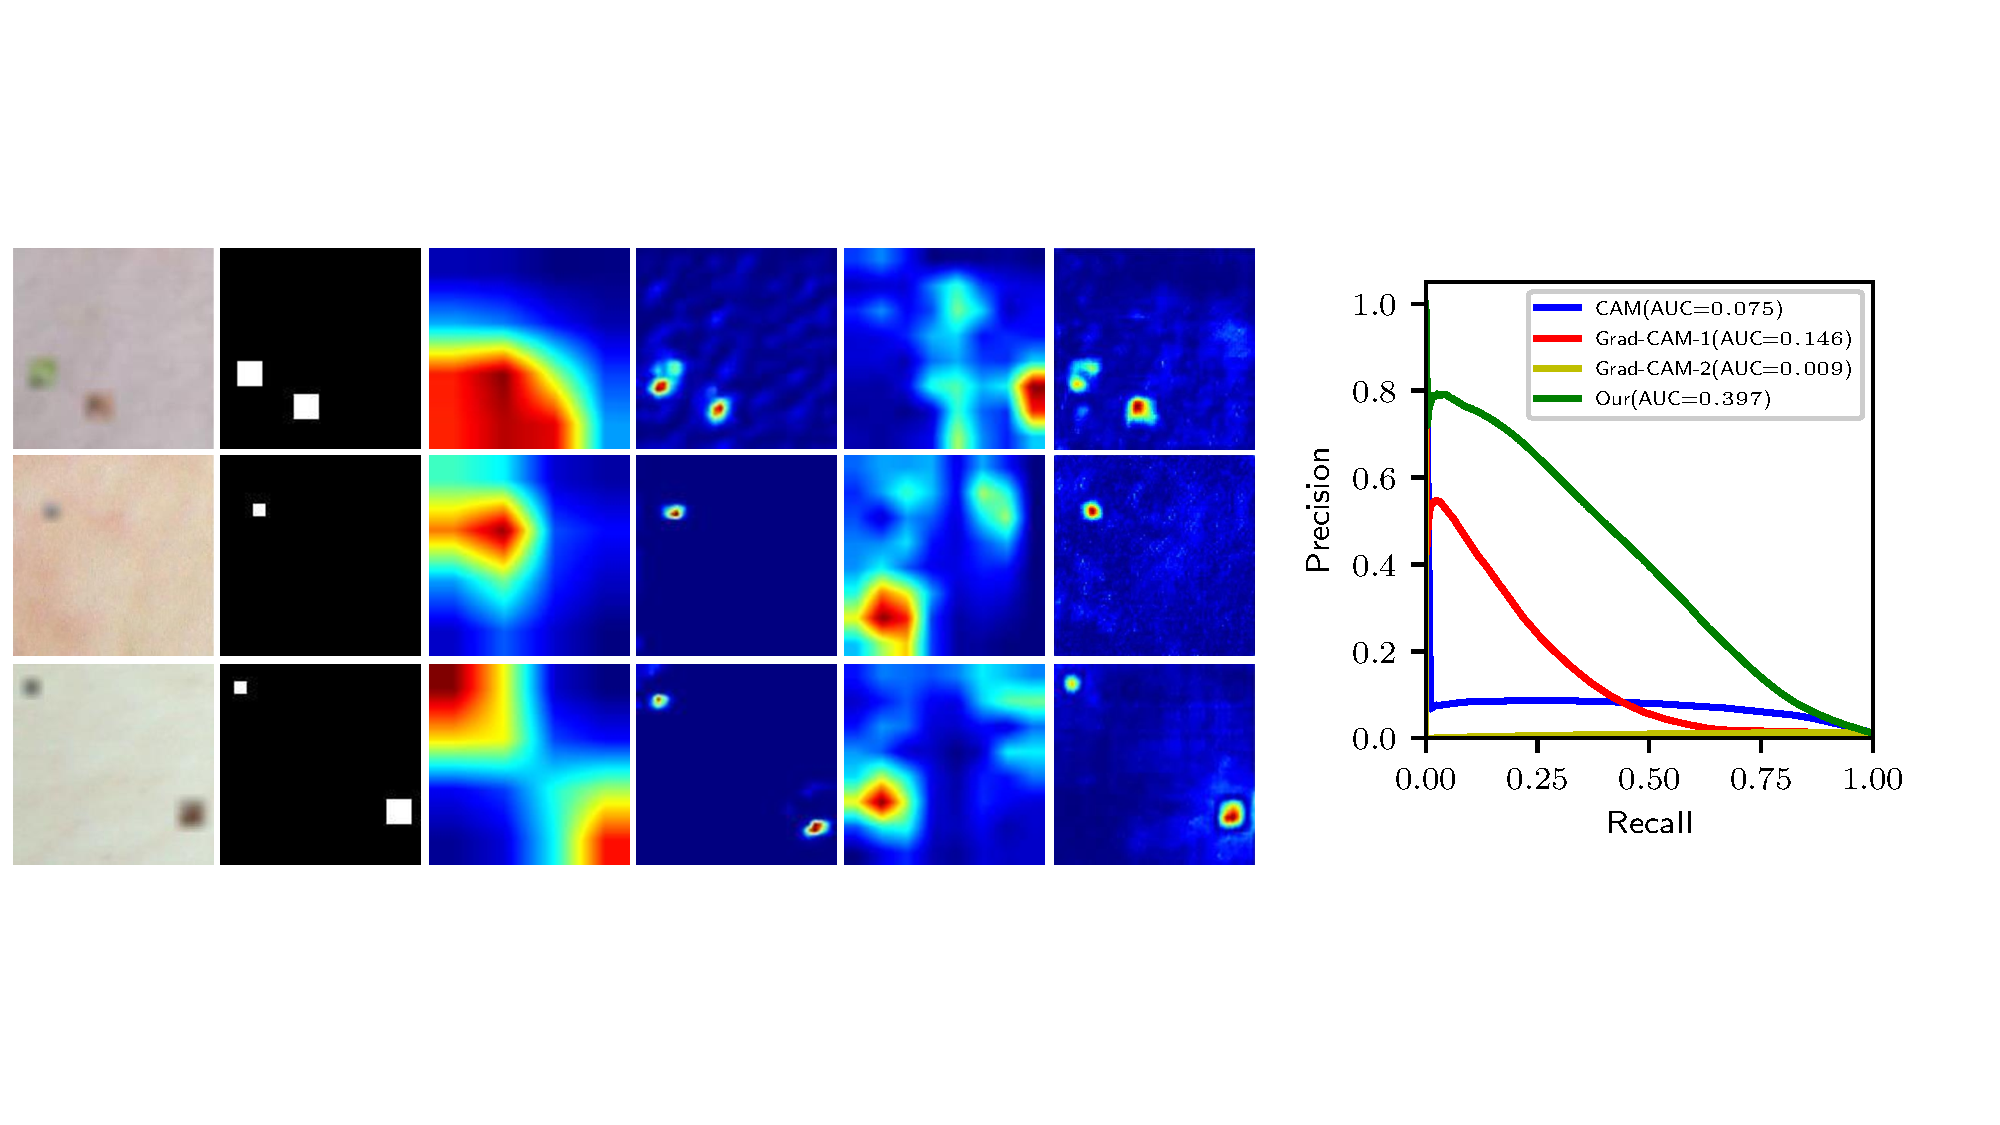
\includegraphics[width=1.0\textwidth]{figure/pr_curve_skin_image.pdf}
	\caption[在二类模拟皮肤病病变数据集上疾病标记物定位热图对比]{在二类模拟皮肤病病变数据集上疾病标记物定位热图对比。} 
	\label{fig:simulated_skin}
\end{figure}

如图\ref{fig:simulated_skin}所示,图中第1列表示原始异常图像,第2列表示其像素级标注,第3列表示CAM得到的定位热图,第4列表示使用Grad-CAM可视化分类器中间卷积层输出的特征图得到的定位热图(记为Grad-CAM-1),第5列表示使用Grad-CAM可视化分类器最后一层卷积层输出的特征图得到的定位热图(记为Grad-CAM-2),第6列是本文提出的模型得到的定位热图。

根据图\ref{fig:simulated_skin},在包含模拟疾病标记物的皮肤图像上的定位热图证实了本文提出的模型的优越性能。从第6列可以看出,本文提出的方法几乎可以完美地、精确地定位了人工模拟的疾病标记物,而CAM(第3列)和Grad-CAM(第4列和第5列)再次表现出了劣势。Grad-CAM作为CAM的泛化,第4列(Grad-CAM-1)中疾病标记物的定位结果明显要比第3列(CAM)更精确、更完美,也就能说明Grad-CAM在定位疾病标记物上的性能优于CAM。同样是由于特征图的过度上采样,CAM(第3列)和Grad-CAM-2(第5列)呈现类似的定位结果:虽然能检测到疾病标记物的位置,但定位结果中也包含了疾病标记物周围的大量正常区域。而Grad-CAM-1(第4列)基本能精确定位到疾病标记物的位置,这是因为Grad-CAM-1是可视化分类器中第一个卷积层的输出特征图来定位疾病标记物,其中上采样倍数较小(64$\times$64 $\rightarrow$ 128$\times$128),这也能从侧面说明在该数据集上定位疾病标记物要比在二类糖尿病性视网膜病变数据集上容易得多(浅层特征便具备高级语义)。
\begin{figure}[h]
	\centering
	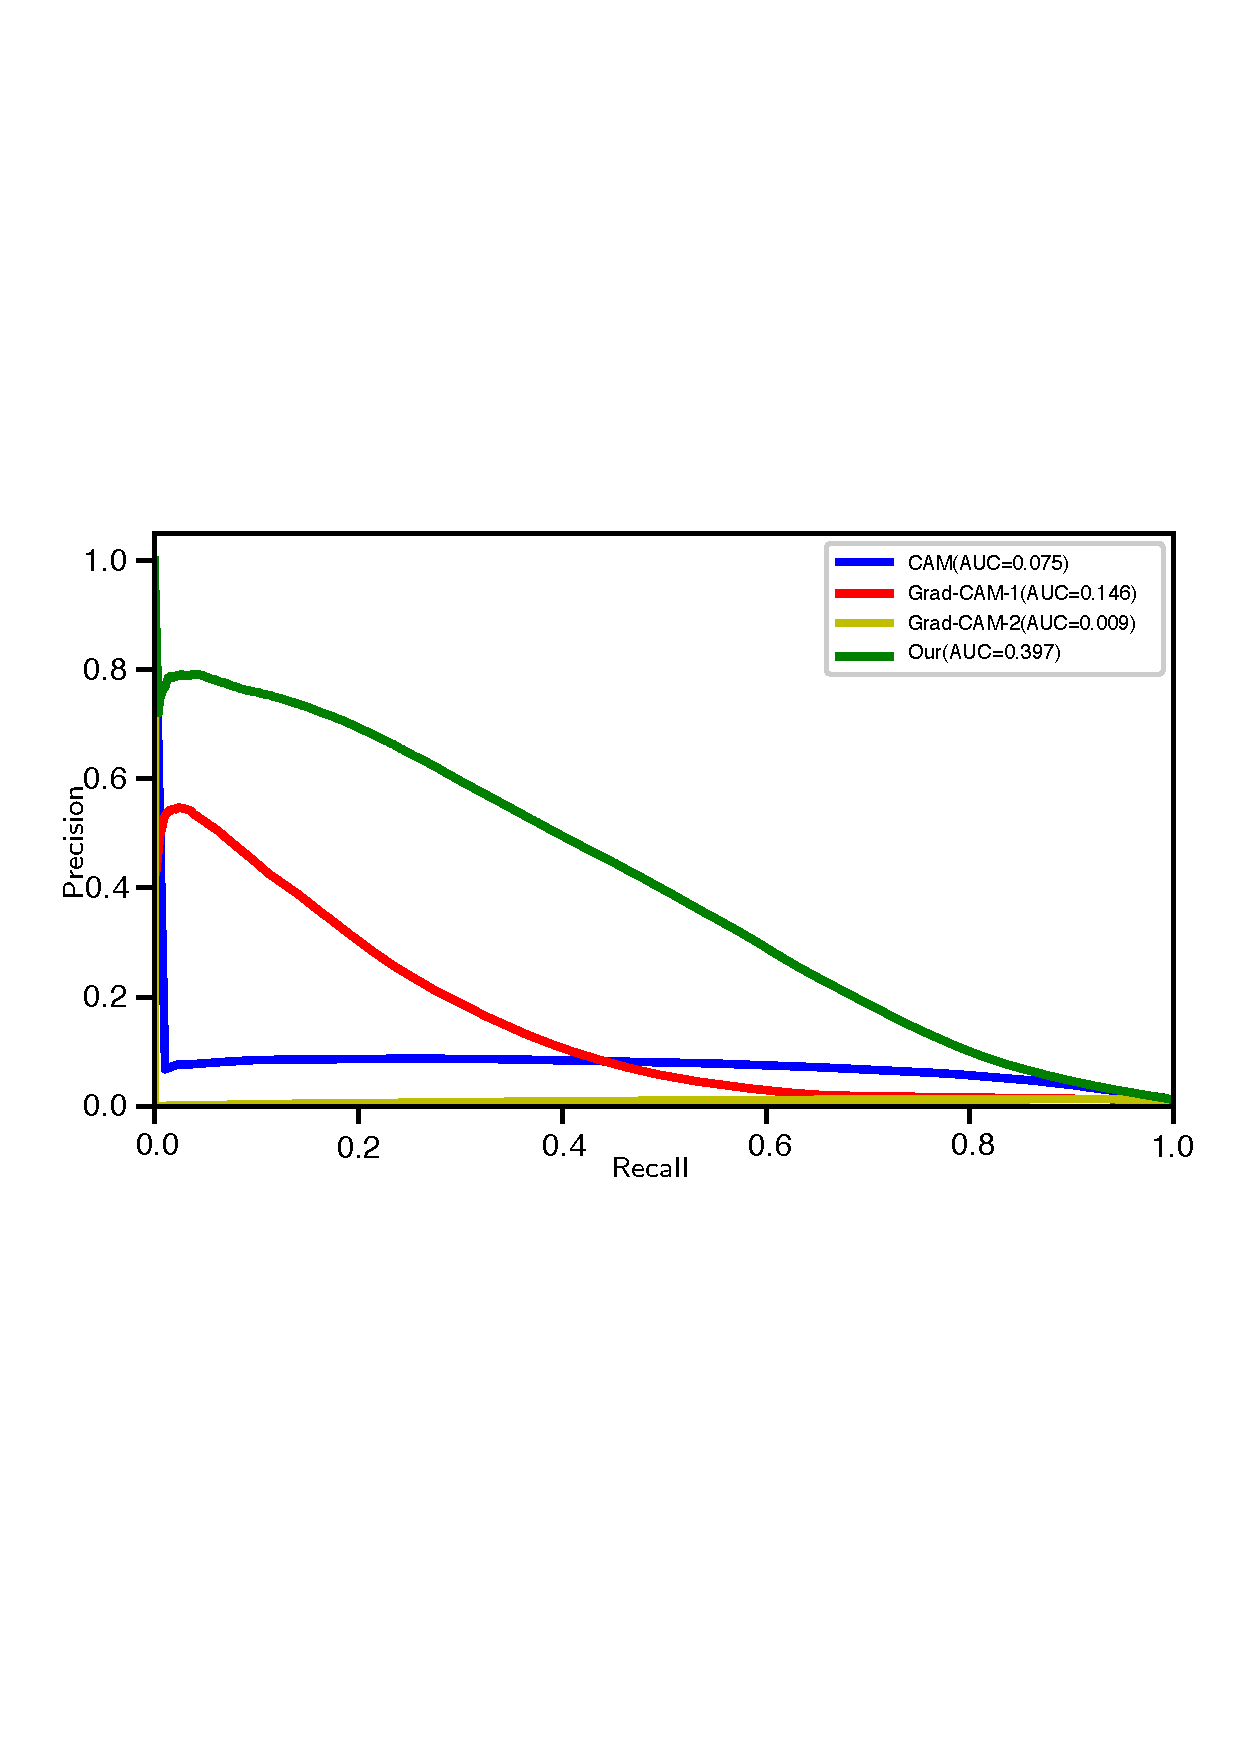
\includegraphics[width=0.7\textwidth]{figure/pr_curve_skin_image/pr_curve.pdf}
	\caption[在二类模拟皮肤病病变数据集上P-R曲线对比]{在二类模拟皮肤病病变数据集上P-R曲线对比。}
	\label{fig:simulated_skin_pr_curve}
\end{figure}

与CAM和Grad-CAM相比,图\ref{fig:simulated_skin}从定性分析的角度证明了本文提出的方法在二类模拟皮肤病病变数据集上的性能优越性,图\ref{fig:simulated_skin_pr_curve}再次从定量分析的角度证明了这一结论。CAM、Grad-CAM-1、Grad-CAM-2和本文提出的模型根据二类模拟皮肤病病变数据集上所有标注所得出的P-R曲线如图\ref{fig:simulated_skin_pr_curve}所示。不难看出,图中绿色曲线明显在其他三条曲线的上方,与下侧横轴和左侧纵轴围成的封闭区域的面积(AUC)上,绿色曲线的AUC分数也明显大于其他三条曲线的AUC,以上四种方法各自对应的P-R曲线的AUC分数分别是0.075、0.146、0.009和0.397。

综上,以上定位热图和P-R曲线均表明了本文提出的方法相较于CAM和Grad-CAM在疾病标记物定位任务上有着更为出色的表现。
\section{CNN分类器和判别器角色探究}\label{sec:g_c_g_d_g_d_c_comparsion}
在\ref{sec:bin_dr_ds_experiment}小节和\ref{sec:bin_simulated_ds_experiment}小节中,本文分别从定性分析和定量分析两个角度在二类糖尿病性视网膜病变数据集和二类模拟皮肤病病变数据集上证明了本文提出的模型在疾病标记物定位任务上的优越性能。为了进一步探究本文提出的模型中各个子模块扮演的角色,本节将设计消融实验,分别去掉本文提出的模型中的CNN分类器和判别器。为了方便后续内容叙述,对于本文提出的模型,本文将其记为G-D-C模型,在此基础上,将移除判别器之后的模型记作G-C模型,将移除CNN分类器之后的模型记作G-D模型。以上三个模型在二类糖尿病性视网膜病变数据集上的定位热图如图\ref{fig:u_d_c_comparation}所示。
\begin{figure}[h]
	\centering
	\includegraphics[width=1.0\textwidth]{figure/u_d_c_comparation.pdf}
	\caption[G-D-C模型、G-C模型和G-D模型定位热图对比]{G-D-C模型、G-C模型和G-D模型在二类糖尿病性视网膜病变数据集上定位热图对比。} 
	\label{fig:u_d_c_comparation}
\end{figure}

如图\ref{fig:u_d_c_comparation}所示,第1列是原始输入图像,其中第一行是正常图像输入,第2-4行是异常图像输入。第2列是G-C模型中编码器-解码器的输出结果,第3列是第2列与第1列的差,也就是G-C模型给出的定位热图,第4列是G-D模型中编码器-解码器的输出结果,第5列是第4列与第1列的差,也就是G-D模型给出的定位热图,第6列是G-D-C模型中编码器-解码器的输出结果,第7列是第6列与第1列的差,也就是G-D-C模型给出的定位热图。第4列图像中的红色框表示其圈出的血管区域与原始输入图像相比发生了改变。

从图\ref{fig:u_d_c_comparation}可以看出,当输入图像是正常图像时(图中第1行),G-D-C模型、G-C模型和G-D模型均能几乎不改变图像中的像素强度,只有在借助图中第5列和第7列的热图才能看出这张正常图像的左上角有些许改变。这说明对于正常图像,以上三种模型均能处理得比较好,以上三种模型的性能差异主要表现在处理异常图像(图中第2-4行)上。不难看出,在没有判别器的情况下(G-C模型),CNN分类器只能帮助编码器-解码器定位了部分疾病标记物(图中第3列热图),而将大部分疾病标记物依然留在了编码器-解码器的输出(图中第2列)中。另一方面,在没有CNN分类器(G-D模型)的情况下,判别器能定位到大部分(如果不是全部的话)的疾病标记物区域(图中第5列)。然而,我们注意到,一些正常区域的像素强度同样也发生了改变(第4列中红色矩形框圈出),也就是说,一些正常的像素被错误地标记为疾病标记物,包括一些血管区域,这种发了生改动的血管区域在第5列的热图中显示得更加突出。相比之下,编码器-解码器与CNN分类器以及判别器的组合(G-D-C模型)不仅可以精确定位大部分的疾病标记物(图中第7列),在编码器-解码器的输出端(第6列)还能标记较少的假阳性疾病标记物(图中第7列热图和第5列热图相比较)和更多的真实疾病标记物(第7列热图和第3列热图相比较)。如\ref{sec:model_architecture_intro}小节描述,这些结果表明CNN分类器和判别器共同帮助编码器-解码器定位并去除疾病标记物。就各自角色而言,CNN分类器在一定程度上帮助帮助编码器-解码器去除疾病标记物(图中第3列),而判别器帮助编码器-解码器进一步去除CNN分类器未能去除的疾病标记物,CNN分类器和判别器共同帮助编码器-解码器彻底去除异常图像中的疾病标记物(图中第7列)。
\begin{figure}[h]
	\centering
	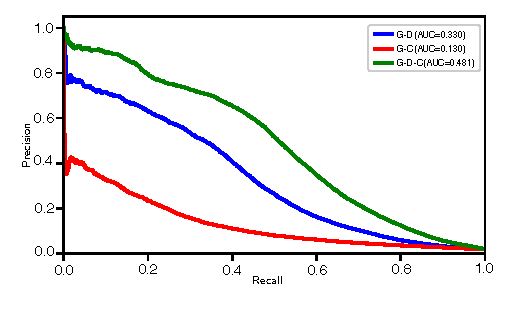
\includegraphics[width=0.7\textwidth]{figure/pr_cureve_u_d_u_c_u_d_c_components.pdf}
	\caption[G-D-C模型、G-C模型和G-D模型P-R曲线对比]{G-D-C模型、G-C模型和G-D模型在40张糖尿病性视网膜病变图像上P-R曲线对比。}
	\label{fig:u_d_c_comparation_pr_curve}
\end{figure}

为了对G-D模型、G-C模型和G-D-C模型进行定量评价,本文再次使用二类糖尿病性视网膜病变数据集中的40张像素级标注图像,再次证实了以上结论。三者的P-R曲线如图\ref{fig:u_d_c_comparation_pr_curve}所示。可以发现,图中绿色P-R曲线在紫色P-R曲线和红色P-R曲线上方。紫色曲线、红色曲线和绿色曲线对应的AUC分别为0.330、0.130和0.481。这些现象再次表明了G-D-C模型定位疾病标记物的性能要优于G-D模型和G-C模型,同时也说明了CNN分类器和判别器的不可或缺性。我们还验证了\ref{sec:idea_thinking}小节中提到的朴素思路,即我们只使用正常图像训练编码器-解码器,希望编码器-解码器具有重建正常信号的能力,从而间接实现疾病标记物的定位。然而,在这40张像素级标注图像上,这种朴素思路得到P-R曲线的AUC为0.083,这远远低于G-C模型、G-D模型和G-D-C模型,这也能说明引入CNN分类器和判别器的必要性。

总之,以上实验结果可以说明CNN分类器和判别器存在的必要性,其中CNN分类器可帮助编码器-解码器尽量去除疾病标记物,判别器进一步帮助编码器-解码器彻底去除疾病标记物,这符合\ref{subsec:model_architecture}小节中我们对二者的角色设计和期望。
%(更为直观的实验数据参见表\ref{tab:baseline_compared_diabetic_ds})
%\begin{table}[h]
%	\centering
%	\caption{基准模型、G-C模型、G-D模型和G-D-C模型在二类视网膜糖尿病病变数据集上的实验结果表。表格展示的是通过P-R曲线计算的AUC分数。}		
%	\label{tab:baseline_compared_diabetic_ds}
%	\begin{tabular}{c|c|c|c|c}
%		\toprule[2pt]
%		模型名称 & 基准模型 & G-C模型 &G-D模型&G-D-C模型 \\
%		\midrule[2pt]
%		AUC	& $0.083$&	$0.130$ & $0.330$ & $\textbf{0.481}$	 \\
%		\bottomrule[2pt]
%	\end{tabular}
%\end{table}

\section{对于经过编码器-解码器的糖尿病性视网膜病变图像的定量分析}\label{sec:indirect_quantitative_evaluation}
在\ref{sec:bin_dr_ds_experiment}小节和\ref{sec:bin_simulated_ds_experiment}小节中,本文在二类模拟皮肤病病变数据集和二类糖尿病性视网膜病变数据集上利用已有的像素级标注图像进行了定量分析,这可看做是一种直接验证的方式。在本节中,我们将从间接角度来再次验证本文提出的模型在处理疾病标记物定位问题的有效性。直观的想法是,在理想情况下,如果一种方法可以准确地定位和去除图像中的疾病标记物,则去除检测到的疾病标记物后的图像将不再包含疾病标记物,那么去除检测到的疾病标记物后的图像将很难与原来的正常图像区分开来。基于以上想法,本文将二类糖尿病性视网膜病变数据集按照80\%和20\%的比例分为训练集和验证集,为下文叙述方便,我们简称该数据集为“原始数据集”,并用训练集数据训练一个ResNet-18二类分类器。随后,对于训练集和验证集,每个图像都被输入到训练之后的编码器-解码器中,所有编码器-解码器的输出图像都被收集起来,从而得到一个新的数据集,为了后文叙述方便,本文将该数据集记为“‘正常’数据集”。最后,本文使用原始数据集训练得到的ResNet-18二类分类器对“正常”数据集分类。在此,为了分别衡量编码器-解码器对异常图像输入的转化能力和对正常图像输入的保持能力,本文使用Recall和Specificity作为分类器的评价标准。相关实验结果如表\ref{tab:quantitative_retinal}所示,前两列表示在原始数据集上的分类结果,后两列表示在“正常”数据集上的分类结果。
\begin{table}[h!]
	\begin{center}
		\caption[ResNet-18二分类器对原始数据集和“正常”数据集分类结果]{ResNet-18二分类器对原始数据集和“正常”数据集的分类结果。} 
		\label{tab:quantitative_retinal}
		\begin{tabular}{c|cc|cc}
			\toprule[2pt]
			& \multicolumn{2}{c|}{原始数据集} & \multicolumn{2}{c}{“正常”数据集} \\
			&  训练集 & 验证集 & 训练集 & 验证集\\
			\midrule[2pt]
			Recall & 0.958 & 0.936 & 0.269 & 0.292\\ \hline
			Specificity & 0.984 & 0.964 & 0.980 & 0.964\\
			\bottomrule[2pt]
		\end{tabular} 
	\end{center}
\end{table}

从表\ref{tab:quantitative_retinal}不难看出,对于原始数据集(表中前两列),ResNet-18分类器不仅在训练集上取得了较高的特异性(Specificity=0.984)和召回率(Recall=0.958),在验证集上也表现了优异性能(Recall和Specificity分别为0.936和0.964),说明ResNet-18分类器已经学会了寻找用于区分疾病标记物的特征。另外,表\ref{tab:quantitative_retinal}中后两列显示,大多数“正常”数据集中的异常图像在训练集和验证集上都被错误地归类为正常,导致更低的召回率(训练集和验证集上的Recall分别为0.269和0.292),说明本文提出的模型能够很好地定位并去除原始异常图像中的疾病标记物,使得ResNet-18二分类器无法将去除疾病标记物的图像与原始正常图像区分开来。另一方面,ResNet-18分类器在正常图像上具有较高的特异性值(训练集和验证集上分别为0.980和0.964),说明经过编码器-解码器后的正常图像仍然被正确分类为正常图像,这证实了编码器-解码器不会改变正常输入,也从实验角度证明了在\ref{sec:idea_thinking}小节中对编码器-解码器的功能设想。总之,在原始数据集和“正常”数据集上,无论对于其中的训练集还是验证集,召回率的大幅下降和特异性的小幅下降都可推断出本文提出的模型可以很好地从图像中去除潜在的疾病标记物,同时保持正常区域不变,从而间接证明了本文提出的方法定位疾病标记物的有效性。
\begin{figure}[h]
	\centering
	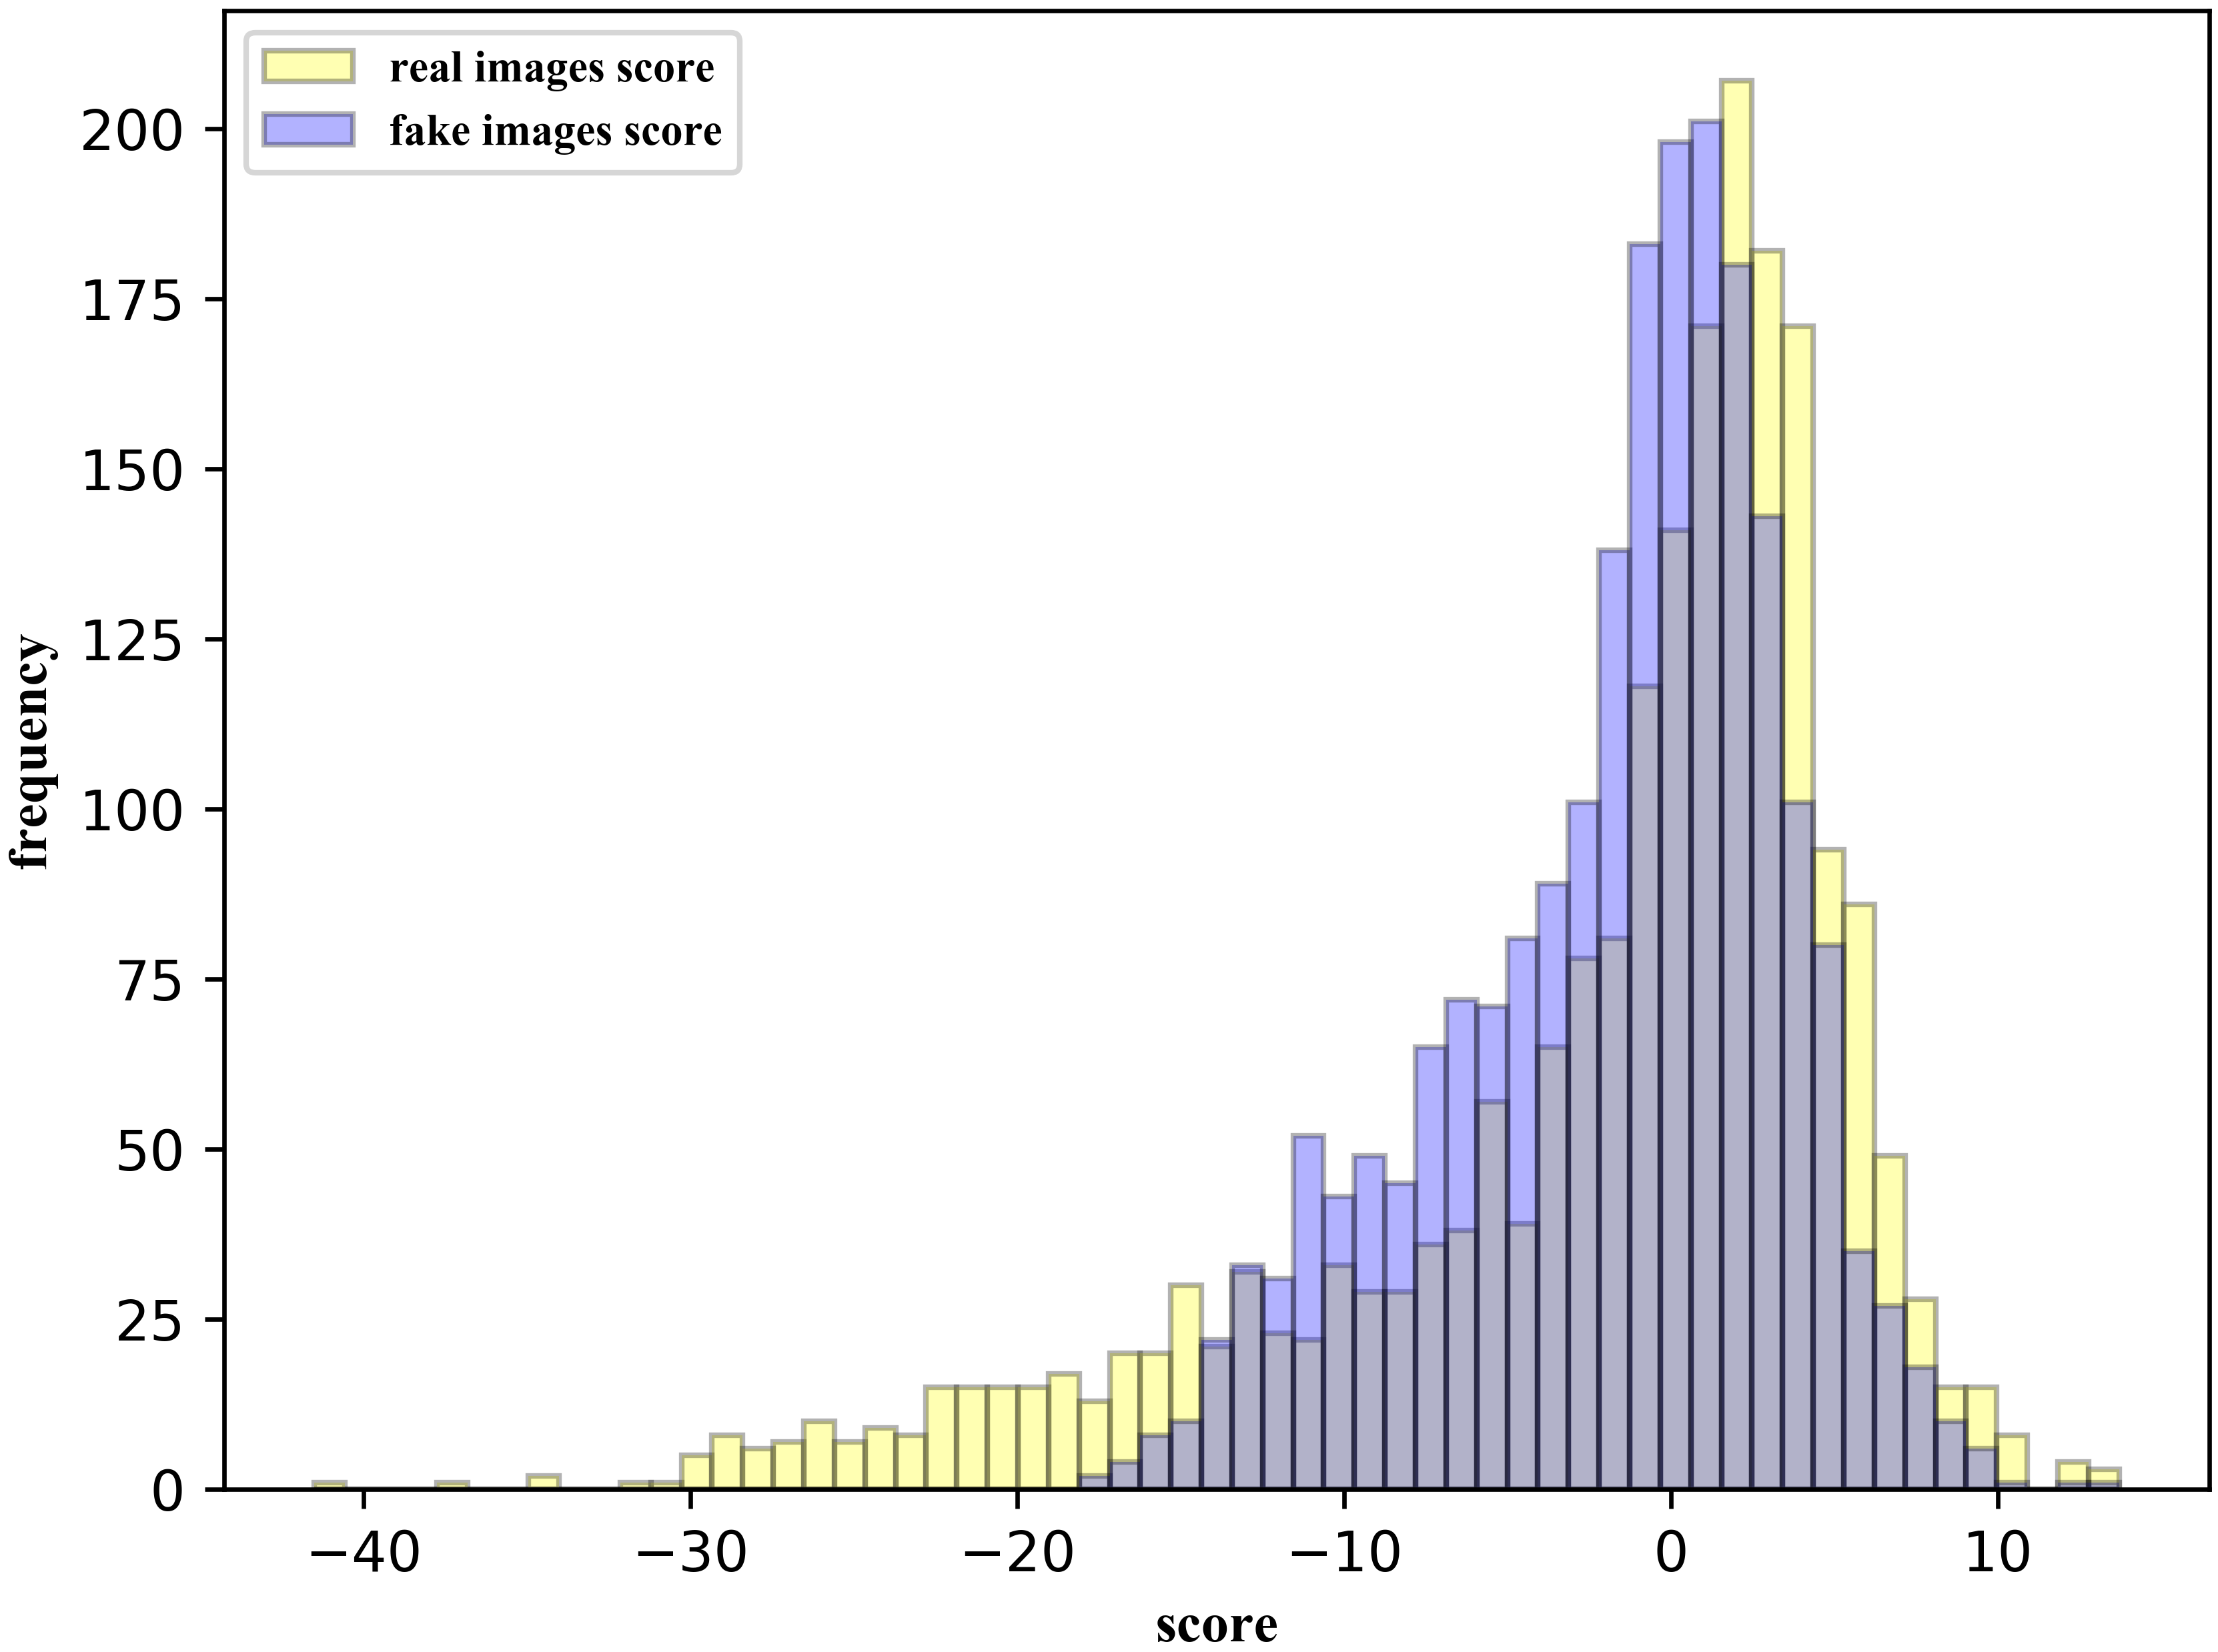
\includegraphics[width=0.9\textwidth]{figure/score_distribution}
	\caption[根据判别器输出分数绘制的频率分布直方图]{根据判别器输出分数绘制的频率分布直方图。二类糖尿病性视网膜病变数据集中的正常图像(真图像)和该数据集中的异常图像经过编码器-解码器之后的输出图像(假图像)作为判别器输入。}
	\label{fig:hist_freq}
\end{figure}

训练结束后,我们还分别将二类糖尿病性视网膜病变数据集中的正常图像(以下简称“真图像”)和该数据集中的异常图像经过编码器-解码器之后的输出图像(以下简称“假图像”)送入判别器,我们根据判别器对真图像和假图像的输出分数所绘制的频率分布直方图如图\ref{fig:hist_freq}所示。图中黄色柱子表示判别器对真图像的输出分数,蓝色柱子表示判别器对假图像的输出分数。可以发现,判别器对真图像的输出分数和假图像的输出分数在频率分布直方图上有较大重叠,如果暂时不考虑横轴中的离群点,判别器对于以上图像的输出分数将会非常接近。我们还可以根据以上直方图计算得到:判别器对于真图像和假图像的平均输出分数分别为-2.1和-1.8,而在初始参数下,判别器对两者的平均输出分数分别为-2.2和-1.0,这说明训练结束后,真图像和假图像之间的相似度得到了极大提升(平均输出分数的差值大大缩小:1.2 $\rightarrow$ 0.3),这可以从判别器角度推断出“正常”数据集中只是存在少量疾病标记物,进而间接说明二类糖尿病性视网膜病变数据集中的疾病标记物已经被本文提出的模型很好地去除。

总之,通过对经过编码器-解码器的糖尿病性视网膜病变图像的定量分析,本小节从额外训练的分类器角度说明本文提出的方法对正常图像输入有较好的保持能力,对异常图像输入有很好的转化能力。从判别器角度说明了本文提出的方法能够不断地提高异常图像经过编码器-解码器之后的输出图像与正常图像的相似度,使得判别器对于真图像和假图像的输出分数不断逼近。这些现象都能间接说明本文提出的方法能够比较好地去除原始数据集中的疾病标记物。
\section{对判别器模型结构的探究}\label{sec:dis_arch}
% 原始 D_FPN
% 对比跨层 D_NSC no skiping connection
% 去掉第一个下采样(高分辨率特征 用中间层 不用高分辨率特征融合) D_NLL no feature map from low layer
% 去掉最后一个下采样(不用中间层特征 只用高分辨率)D_NML no feature map from middle layer
在本节内容中,在保持其他设置不变的情况下,本文设置了一系列消融实验来探究不同判别器结构对于定位疾病标记物的影响。为了后文叙述方便,本文将默认判别器记作$\mathrm{D}_\mathrm{FPN}(i,j)$,其中二元组$(i,j)$表示判别器中卷积层总数为$i$,其中前$j$个为下采样卷积层,例如,$\mathrm{D}_\mathrm{FPN}(\mathrm{7},\mathrm{4})$表示一个总共有7个卷积层,其中前4个为下采样卷积层的判别器,这也是本章所有实验的默认判别器网络结构(对应网络结构见图\ref{subfig:discrimintor_architecture})。对于默认判别器,本文将去掉所有跨层结构的判别器记作$\mathrm{D}_\mathrm{NSC}(i,j)$。在默认判别器中,最后一个全连接层的输入是由第一个下采样卷积层的输出特征、最后一个下采样卷积层的输出特征和最后一个卷积层的输出特征进行特征融合得到,本文将去掉第一个下采样卷积层特征输出而进行特征融合的判别器记作$\mathrm{D}_\mathrm{NLL}(i,j)$,将去掉最后一个下采样卷积层输出特征而进行特征融合的判别器记作$\mathrm{D}_\mathrm{NML}(i,j)$,以上二元组$(i,j)$的含义均相同。我们在保持其他实验设置不变的情况,按照上述判别器结设置构依次在二类模拟皮肤病病变数据集上进行测试,根据实验结果绘制的P-R曲线如图\ref{fig:pr_curve_skin_dis_arch}所示。
\begin{figure}[h]
	\centering
	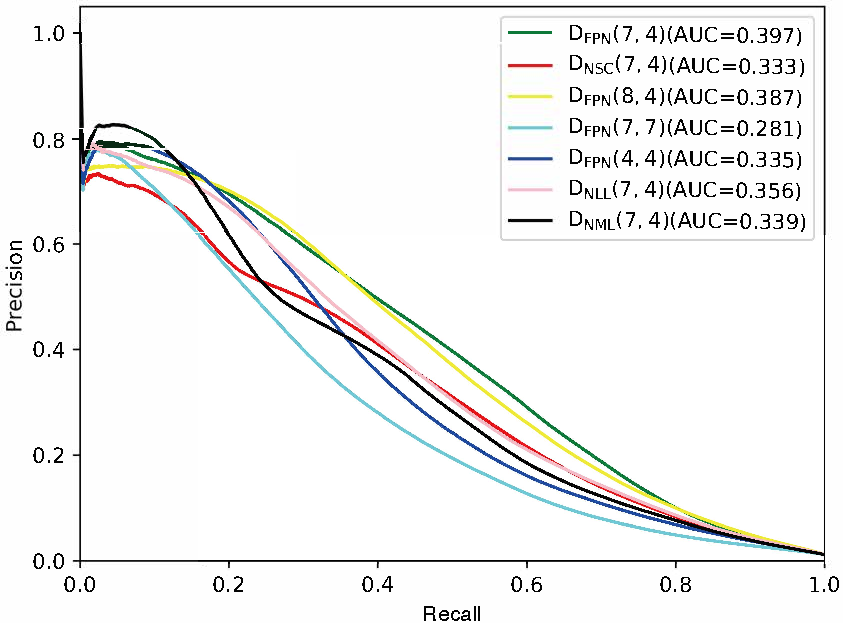
\includegraphics[width=0.7\textwidth]{figure/pr_curve_dis_arch/pr_curve.pdf}
	\caption[不同判别器模型结构下P-R曲线对比]{在二类模拟皮肤病病变数据集上,不同判别器模型结构下P-R曲线对比。} 
	\label{fig:pr_curve_skin_dis_arch}
\end{figure}

从上图可以看出,对于默认判别器模型$\mathrm{D}_\mathrm{FPN}(\mathrm{7},\mathrm{4})$(图中绿色曲线),本文提出的模型定位性能最佳,AUC分数最高(AUC=0.397)。相比较之下,当去掉默认判别器所有跨层连接时($\mathrm{D}_\mathrm{NSC}(7,4)$,图中红色曲线),性能下降最为严重(0.397 $\rightarrow$ 0.333),这主要是因为网络提取到的浅层高分辨率特征往往对异常图像中尺寸偏小的疾病标记物有极强语义性。另外,在原始判别器基础上,我们去掉最后一个下采样卷积层与最后一个全连接层的跨层连接得到$\mathrm{D}_\mathrm{NML}(\mathrm{7},\mathrm{4})$(图中黑色曲线),同理,我们去掉第一个下采样卷积层与最后一个全连接层的跨层连接得到$\mathrm{D}_\mathrm{NLL}(\mathrm{7},\mathrm{4})$(图中粉色曲线),在以上两种情况下,虽然本文提出的模型的定位性能也有所下降,前者AUC:0.397 $\rightarrow$ 0.339,后者AUC:0.397 $\rightarrow$ 0.356,但是两者AUC分数的下降幅度与$\mathrm{D}_\mathrm{NSC}(\mathrm{7},\mathrm{4})$相比都要小($\mathrm{D}_\mathrm{NSC}(\mathrm{7},\mathrm{4})$、$\mathrm{D}_\mathrm{NML}(\mathrm{7},\mathrm{4})$和$\mathrm{D}_\mathrm{NLL}(\mathrm{7},\mathrm{4})$相较于默认判别器模型,AUC分数下降幅度分别为0.064,0.058和0.041),也进一步说明判别器模型的浅层特征和中间层特征对于定位异常图像中分布广泛、大小不一的疾病标记物的重要性,这也是我们在判别器模型中加入跨层结构,让判别器融合不同层次、不同分辨率的特征的主要原因。我们还能发现,$\mathrm{D}_\mathrm{NML}(\mathrm{7},\mathrm{4})$的AUC下降相较于$\mathrm{D}_\mathrm{NLL}(\mathrm{7},\mathrm{4})$较大,这说明中间层特征相比浅层特征对定位模拟皮肤病病变图像中的疾病标记物而言更加重要。另外,在默认判别器$\mathrm{D}_\mathrm{FPN}(\mathrm{7},\mathrm{4})$基础上再加入一个卷积层可得到$\mathrm{D}_\mathrm{FPN}(\mathrm{8},\mathrm{4})$(图中黄色曲线),但就定位性能来看AUC分数出现了略微下降(AUC分数为0.387),这是因为额外引入一个卷积层虽然没有改变特征图的尺寸,但是更深的网络意味着梯度的回传也会更加困难。另外,本文针对判别器下采样的次数,本文也设置了相关实验,当判别器模型采用$\mathrm{D}_\mathrm{FPN}(\mathrm{7},\mathrm{7})$(图中青色曲线)时,我们发现本文提出的模型的定位性能最差(AUC=0.281)。这是因为输入图像尺寸为128$\times$128(实际上判别器的下采样次数最多为7次),随着下采样次数增加,特征图分辨率不断减少,在此过程中,相较于像素数量占绝对优势的正常像素,尺寸较小的疾病标记物的相关信息更难以被提取到,导致本该具备高语义的低分辨率高层特征对于尺寸较小的疾病标记物来说,其语义性大打折扣。反之,当下采样次数过少时,此时的低分辨率的高层特征中往往包含很多冗余或者无关干扰信息,故此时高层特征的语义性实际上也较差,这也是判别器模型采用$\mathrm{D}_\mathrm{FPN}(\mathrm{4},\mathrm{4})$时,其AUC分数(图中蓝色曲线,AUC=0.335)相较于默认判别器模型也有所下降的原因。

总之,这些实验结果均说明了本文判别器中引入跨层结构的必要性,还说明了判别器在深度过大或者下采样次数过多时对于定位疾病标记物的不利影响。

%为了更为直观看出以上各个模型之间的定位性能差异,我们将以上判别器模型结构及其AUC分数列在表\ref{tab:dis_arch}中。
%\begin{table}[h]
%	\centering
%	\caption{不同超参数组合下,本文提出的模型在二类视网膜糖尿病病变数据集上计算得到的AUC分数列表。}		
%	\label{tab:dis_arch}
%	\resizebox{1.0\textwidth}{!}{
%		\begin{tabular}{c|c|c|c|c|c|c|c}
%			\toprule[2pt]
%			& $\mathrm{D}_\mathrm{FPN}(7,4)$ & $\mathrm{D}_\mathrm{NSC}(7,4)$&
%			$\mathrm{D}_\mathrm{NLL}(7,4)$&
%			$\mathrm{D}_\mathrm{NML}(7,4)$& $\mathrm{D}_\mathrm{FPN}(8,4)$&
%			$\mathrm{D}_\mathrm{FPN}(7,7)$&
%			$\mathrm{D}_\mathrm{FPN}(4,4)$ \\
%			\midrule[2pt]
%			AUC	& $\textbf{0.397}$ &	$0.333 $ & $0.356$ & $0.339$ & $0.387$& $0.281$ & $0.335$	 \\
%			\bottomrule[2pt]
%		\end{tabular}
%	}
%\end{table}

\section{不同超参数下的实验结果分析}\label{sec:hyper_paras}
为了验证本文提出的模型的超参数鲁棒性(损失函数见等式\ref{equ:model_loss_func}),本文对损失函数中的两个超参数$\lambda_{1}$和$\lambda_{2}$进行测试,旨在找出比较鲁邦的超参数范围。为此,在保证学习率、迭代次数、网络参数初始化等所有相关设置不变的情况下,本文取了7种不同$\lambda_{1}$和$\lambda_{2}$超参数取值,在二类糖尿病性视网膜病变数据集上进行了相关测试。这里同样使用P-R曲线及其AUC分数作为评价标准。根据40张像素级标注图像,本文绘制的P-R曲线如图\ref{fig:pr_curve_retinal_hyper_paras}所示。
\begin{figure}[h]
	\centering
	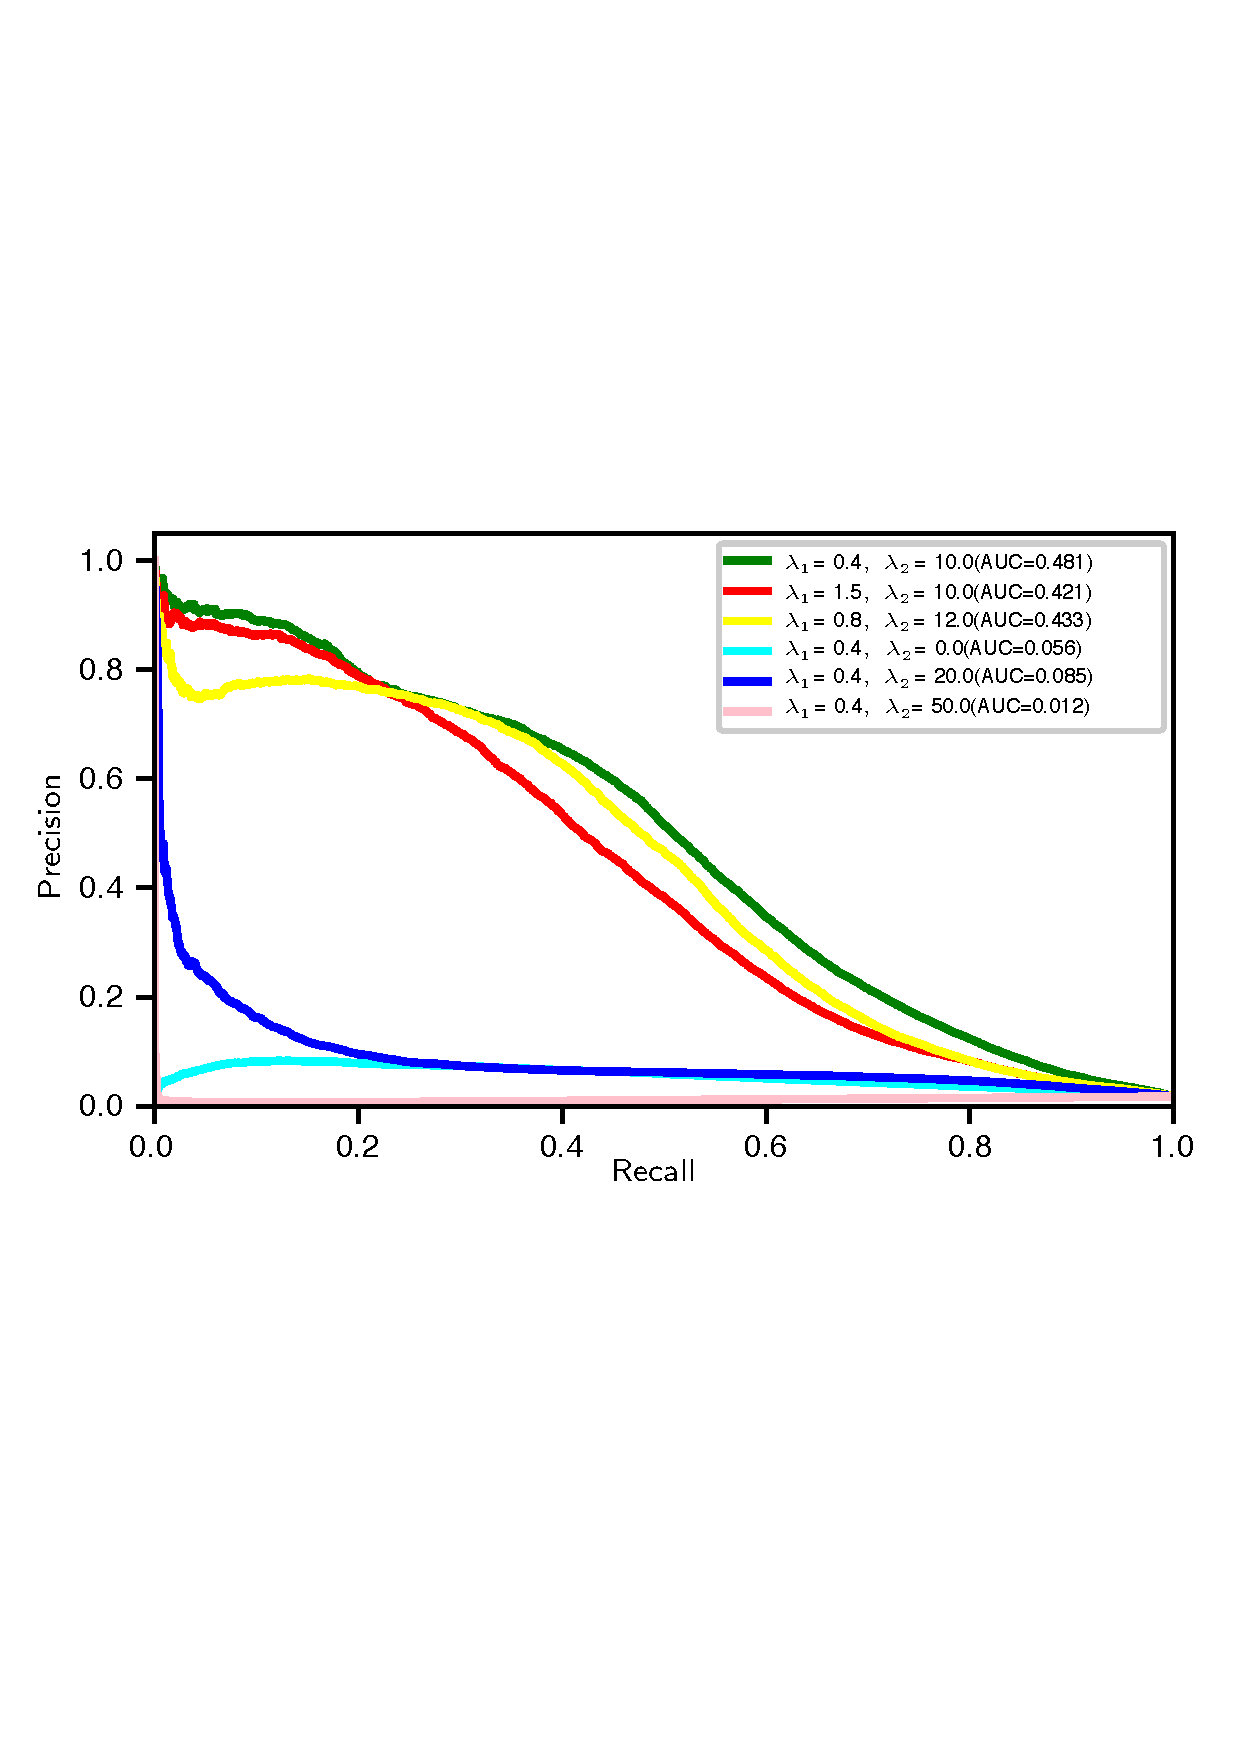
\includegraphics[width=0.7\textwidth]{figure/pr_curve_retinal_hyper_paras/pr_curve.pdf}
	\caption[不同超参数组合下P-R曲线对比]{在40张糖尿病性视网膜病变图像上,不同超参数组合下P-R曲线对比。}
	\label{fig:pr_curve_retinal_hyper_paras}
\end{figure}

从图\ref{fig:pr_curve_retinal_hyper_paras}可以看出,在$\lambda_{1}$=0.4,$\lambda_{2}$=10(默认超参数)、$\lambda_{1}$=1.5,$\lambda_{2}$=10和$\lambda_{1}$=0.8,$\lambda_{2}$=12这三组超参数设置下,AUC分数分别为0.481(图中绿色曲线)、0.421(图中深红色曲线)和0.433(图中黄色曲线),这可以说明默认参数下本文提出的方法表现最佳,也表明当$\lambda_{1}\in$ [0.4,1.5],$\lambda_{2}\in$ [10,12]时,文本提出的模型的性能比较稳定。另外,注意到$\lambda_{2}$=0时,本文提出的模型取得较低AUC分数(AUC=0.056,图中青色曲线),这是因为当$\lambda_{2}$=0时本文提出的方法在训练过程中没有了L1损失函数对编码器-解码器的约束,这导致本文提出的方法在去除疾病标记物的同时也不可避免地改变了正常区域,说明了L1损失函数对编码器-解码器的约束的必要性。而当$\lambda_{2}\geq$ 20时,本文提出的模型定位疾病标记物的性能也比较差,比如,$\lambda_{2}$=20时,AUC分数为0.085(图中蓝色曲线);$\lambda_{2}$=50时,AUC分数为0.012(图中品红色曲线),这是因为当$\lambda_{2}$过大时,在损失函数中起主导作用的是L1损失函数,此时,无论对于异常图像还是正常图像输入,编码器-解码器的输出相较于输入变化均较小,否则L1损失函数将会给予较大惩罚,最终导致疾病标记物定位失败,表现出AUC分数较低。而另一个极端,当$\lambda_{1}$=0时,相当于模型中移去CNN分类器,此时本文提出的方法与G-D模型一致,AUC为0.330(见图\ref{fig:u_d_c_comparation_pr_curve}中紫色P-R曲线)。

以上P-R曲线表明了本文提出的方法对于超参数$\lambda_{1}$和$\lambda_{2}$具有较好的鲁棒性。超参数$\lambda_{1}$和$\lambda_{2}$在极端情况(过大或者过小)下,本文提出的方法的定位性能会出现不同程度的下降,这也符合我们的预期。
%\begin{table}[h]
%	\centering
%	\caption{不同超参数组合下,本文提出的模型在二类视网膜糖尿病病变数据集上计算得到的AUC分数列表。}		
%	\label{tab:diff_parameters}
%	\resizebox{1.0\textwidth}{!}{
%		\begin{tabular}{c|c|c|c|c|c|c}
%			\toprule[2pt]
%			& $\lambda_{1}=0.4,\lambda_{2}=10$ & $\lambda_{1}=0.8, \lambda_{2}=10$& $\lambda_{1}=1.5, \lambda_{2}=10$&
%			$\lambda_{1}=0.4,\lambda_{2}=0$& $\lambda_{1}=0.4,\lambda_{2}=20$ & $\lambda_{1}=0.4,\lambda_{2}=50$ \\
%			\midrule[2pt]
%			AUC	& $\textbf{0.481}$ &	$0.421 $ & $0.433$ & $0.056$ & $0.085$& $0.012$	 \\
%			\bottomrule[2pt]
%		\end{tabular}
%	}
%\end{table}
\section{本章小结}
本章主要展示了在二类糖尿病性视网膜病变数据集和二类模拟皮肤病病变数据集上的相关实验结果及其分析,与CAM和Grad-CAM相比,从P-R曲线及其AUC角度看,本文提出的模型可以更为精确地定位疾病标记物。另外,为了让读者更清楚地理解本文提出的模型的内部情况,本章设计了系列消融实验,例如,在\ref{sec:g_c_g_d_g_d_c_comparsion}小节中通过分别去掉CNN分类器和判别器的方式来探究二者在完整模型中所起到的作用。除了直接与CAM和Grad-CAM作比较来证明本文提出的模型的性能优越性,我们还通过间接方式分别从额外训练的分类器和本文提出的模型中的判别器进行了进一步验证(参见\ref{sec:indirect_quantitative_evaluation}小节)。最后,本章还分别设计了两组对比实验分别探究了本文提出的模型的适用超参数范围和判别器结构变化对于整体模型的影响。到此,本文提出的模型在二类疾病标记物定位问题上的叙述完毕。接下来将在第\ref{sec:multi_classes}章中展示多类疾病标记物定位问题的相关实验结果。如\ref{sec:existing_diffcuities}小节中所描述的那样,由二类疾病标记物定位问题扩展到多类疾病标记物定位问题并不是一个简单的二类到多类的推广,而是存在诸多难题。在数据集方面,图像数量比较多、图像质量比较高的多类数据集难以收集,而且图像的像素级标注代价高昂的问题依然存在。在模型的训练方面,对于CNN分类器的处理比较容易,将二类交叉熵损失替换成多类交叉熵损失即可,难点是如何处理判别器,因为生成对抗网络只有真/假图像两个输入端,是否要添加新的判别器来处理新加入的类别。当有多个类别存在时,如何加载训练数据,这些均是值得考虑的问题。接下来,在第\ref{sec:multi_classes}章中,本文围绕以上问题展开叙述,随后展示相关实验结果并对其进行分析。


